\documentclass[12pt,utf8,notheorems,compress,t]{beamer}
\usepackage{etex}

\usepackage[english]{babel}

\usepackage{mathtools}
\usepackage{booktabs}
\usepackage{array}
\usepackage{ragged2e}
\usepackage{multicol}
\usepackage{tabto}
\usepackage{xstring}
\usepackage{mathtools}
\usepackage{soul}\setul{0.3ex}{}
\usepackage[all]{xy}
\xyoption{rotate}
\usepackage{tikz}
\usetikzlibrary{calc,shapes.callouts,shapes.arrows}
\hypersetup{colorlinks=true}

\usepackage[protrusion=true,expansion=true]{microtype}

\setlength\parskip{\medskipamount}
\setlength\parindent{0pt}

\title{Using the internal language of toposes in algebraic geometry}
\author{Ingo Blechschmidt}
\date{May 24th, 2016}

\usetheme{Warsaw}
\usecolortheme{seahorse}
%\usefonttheme{default}?
%\usepackage{kurier}?
\usefonttheme{serif}
\usepackage[T1]{fontenc}
\usepackage{libertine}
%\usepackage{mathpazo}
\useinnertheme{rectangles}

\newcommand{\A}{\mathcal{A}}
\renewcommand{\AA}{\mathbb{A}}
\newcommand{\E}{\mathcal{E}}
\newcommand{\F}{\mathcal{F}}
\renewcommand{\G}{\mathcal{G}}
\newcommand{\GG}{\mathbb{G}}
\renewcommand{\O}{\mathcal{O}}
\newcommand{\K}{\mathcal{K}}
\newcommand{\NN}{\mathbb{N}}
\newcommand{\RR}{\mathbb{R}}
\newcommand{\PP}{\mathbb{P}}
\newcommand{\ZZ}{\mathbb{Z}}
\renewcommand{\P}{\mathcal{P}}
\newcommand{\ppp}{\mathfrak{p}}
\newcommand{\defeq}{\vcentcolon=}
\newcommand{\defeqv}{\vcentcolon\equiv}
\newcommand{\Sh}{\mathrm{Sh}}
\newcommand{\GL}{\mathrm{GL}}
\newcommand{\Zar}{\mathrm{Zar}}
\newcommand{\op}{\mathrm{op}}
\newcommand{\Set}{\mathrm{Set}}
\newcommand{\Sch}{\mathrm{Sch}}
\newcommand{\LRS}{\mathrm{LRS}}
\newcommand{\Hom}{\mathrm{Hom}}
\DeclareMathOperator{\Spec}{Spec}
\newcommand{\lra}{\longrightarrow}
\newcommand{\RelSpec}{\operatorname{\text{\ul{$\mathrm{Spec}$}}}}
\renewcommand{\_}{\mathpunct{.}}
\newcommand{\?}{\,{:}\,}
\newcommand{\speak}[1]{\ulcorner\text{\textnormal{#1}}\urcorner}
\newcommand{\ull}[1]{\underline{#1}}
\newcommand{\affl}{\ensuremath{{\ull{\AA}^1_S}}}
\newcommand{\Ll}{\vcentcolon\!\Longleftrightarrow}

\setbeamertemplate{blocks}[rounded][shadow=false]

\newcommand{\fmini}[2]{\framebox{\begin{minipage}{#1}#2\end{minipage}}}
\makeatletter
\def\underunbrace#1{\mathop{\vtop{\m@th\ialign{##\crcr
      $\hfil\displaystyle{#1}\hfil$\crcr\noalign{\kern3\p@\nointerlineskip}
      \crcr\noalign{\kern3\p@}}}}\limits}
\def\overunbrace#1{\mathop{\vbox{\m@th\ialign{##\crcr\noalign{\kern3\p@}
      \crcr\noalign{\kern3\p@\nointerlineskip}
      $\hfil\displaystyle{#1}\hfil$\crcr}}}\limits}
\makeatother

\newenvironment{changemargin}[2]{%
  \begin{list}{}{%
    \setlength{\topsep}{0pt}%
    \setlength{\leftmargin}{#1}%
    \setlength{\rightmargin}{#2}%
    \setlength{\listparindent}{\parindent}%
    \setlength{\itemindent}{\parindent}%
    \setlength{\parsep}{\parskip}%
  }%
  \item[]}{\end{list}}

\newcommand{\pointthis}[2]{%
  \tikz[remember picture,baseline]{\node[anchor=base,inner sep=0,outer sep=0]%
    (#1) {#1};\node[overlay,rectangle callout,%
    callout relative pointer={(-0.5cm,0.8cm)},fill=blue!20] at ($(#1.north)+(1.1cm,-1.4cm)$) {#2};}%
}%

\newcommand{\hcancel}[5]{%
  \tikz[baseline=(tocancel.base)]{
    \node[inner sep=0pt,outer sep=0pt] (tocancel) {#1};
    \draw[red, line width=0.4mm] ($(tocancel.south west)+(#2,#3)$) -- ($(tocancel.north east)+(#4,#5)$);
  }%
}

\newcommand{\slogan}[1]{%
  \begin{center}%
    \setlength{\fboxrule}{2pt}%
    \setlength{\fboxsep}{8pt}%
    {\usebeamercolor[fg]{item}\fbox{\usebeamercolor[fg]{normal text}\parbox{0.84\textwidth}{#1}}}%
  \end{center}%
}

\newcommand{\sloganwithoutborder}[1]{%
  \begin{center}%
    \setlength{\fboxrule}{0pt}%
    \setlength{\fboxsep}{-14pt}%
    {\usebeamercolor[fg]{item}\fbox{\usebeamercolor[fg]{normal
    text}\parbox{0.9\textwidth}{\begin{center}#1\end{center}}}}%
  \end{center}%
}


\setbeamertemplate{frametitle}[default][colsep=-2bp,rounded=false,shadow=false,center]

\setbeamertemplate{headline}{}
\setbeamertemplate{navigation symbols}{}

\newcounter{framenumberpreappendix}
\newcommand{\backupstart}{
  \setcounter{framenumberpreappendix}{\value{framenumber}}
}
\newcommand{\backupend}{
  \addtocounter{framenumberpreappendix}{-\value{framenumber}}
  \addtocounter{framenumber}{\value{framenumberpreappendix}} 
}

\setbeamertemplate{footline}{%
  \begin{beamercolorbox}[wd=\paperwidth,ht=2.5ex,dp=1.25ex,right,rightskip=1mm,leftskip=1mm]{frametitle right}
    {\quad} \inserttitle \hfill
    \insertframenumber\,/\,\inserttotalframenumber {\quad}
  \end{beamercolorbox}}

\newcommand{\hil}[1]{{\usebeamercolor[fg]{item}{\textbf{#1}}}}

\IfSubStr{\jobname}{\detokenize{nonotes}}{
  \setbeameroption{hide notes}
}{
  \setbeameroption{show notes}
}
\setbeamertemplate{note page}[plain]

\begin{document}

\addtocounter{framenumber}{-1}

\begin{frame}[c]
  \centering
  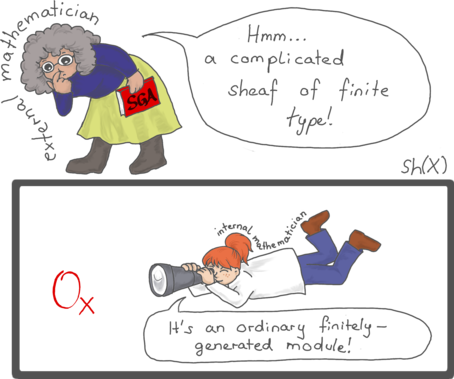
\includegraphics[scale=0.3]{images/external-internal-small}
  \medskip

  \hil{Using the internal language of toposes in \\ algebraic geometry}
  \medskip

  \scriptsize
  Ingo Blechschmidt \\
  University of Augsburg
  \medskip

  Category Theory Seminar \\
  Centre for Mathematical Sciences \\
  University of Cambridge \\
  \ \\
  May 24th, 2016
  \par
\end{frame}

\backupstart
{\usebackgroundtemplate{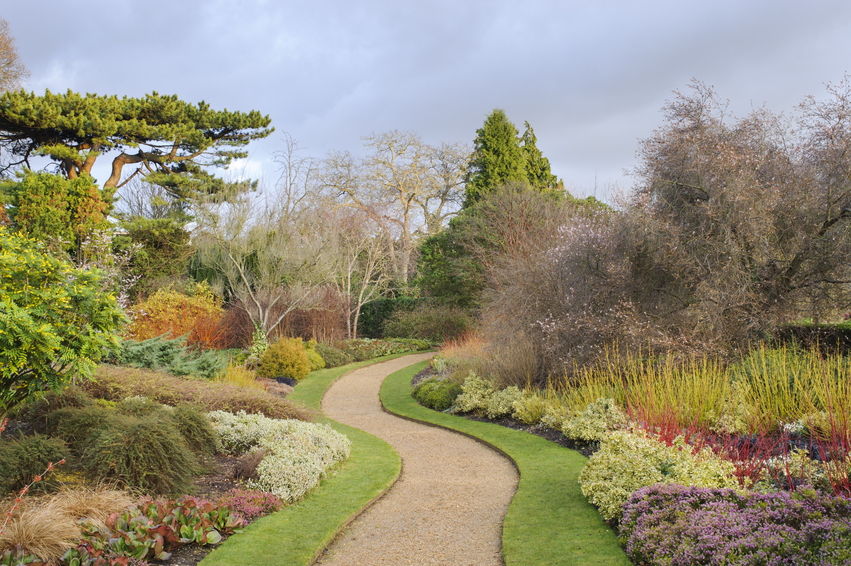
\includegraphics[width=\paperwidth]{images/cambridge-university-botanic-garden}}
\begin{frame}[plain]
  \vspace{\textheight}\vspace{-1em}
  \centering
  \emph{Cambridge University Botanic Garden} \\
  \par
\end{frame}}

\note{
  Photo source:
  \href{http://www.stpaulscambridge.org.uk/classes-and-room-hire/activities-and-events/newtown-news/}{Newtown
  News}
}

\frame[t]{\frametitle{Outline}\scriptsize\begin{itemize}\item[]\tableofcontents\end{itemize}}
\backupend

\note{\justifying\fontsize{8pt}{9.6}\selectfont
  \begin{center}\large\textbf{Abstract}\end{center}

  \begin{changemargin}{2.5em}{2.5em}
    We describe how the internal language of certain
    toposes, the associated small and big Zariski toposes of a scheme, can be
    used to give simpler definitions and more conceptual proofs of the basic
    notions and observations in algebraic geometry.
    % This is useful for studying schemes from a local or relative point of view.

    The starting point is that, from the internal point of view, sheaves of rings
    and sheaves of modules look just like plain rings and plain modules.
    In this way, some concepts and statements of scheme theory can be reduced to
    concepts and statements of intuitionistic linear algebra.

    Furthermore, modal operators can be used to model phrases such as ``on a
    dense open subset it holds that'' or ``on an open neighbourhood of a given
    point it holds that''. These operators define certain subtoposes; a
    generalization of the double-negation translation is useful in order to
    understand the internal universe of those subtoposes from the internal point
    of view of the ambient topos.

    A particularly interesting task is to internalise the
    construction of the relative spectrum, which, given a quasicoherent sheaf of algebras
    on a scheme~$X$, yields a scheme over~$X$. From the internal point of
    view, this construction should simply reduce to an intuitionistically sensible
    variant of the ordinary construction of the spectrum of a ring, but it turns
    out that this expectation is too naive and that a refined approach is
    necessary.

    We also discuss how the little Zariski topos can be described using the
    internal language of the big Zariski topos, and vice versa; here too there
    is a small surprise.
  \end{changemargin}
}


\section{Basics}

\subsection{What is a scheme?}

\begin{frame}\frametitle{What is a scheme?}
  \begin{itemize}
  \item A \hil{manifold} is a space which is \hil{locally isomorphic} to some open
  subset of some~$\RR^n$.
  \medskip
  \item A \hil{scheme} is a space which is \hil{locally isomorphic} to the
  \hil{spectrum of some (commutative) ring}:
  \[ \Spec A \defeq \{ \ppp \subseteq A \,|\, \text{$\ppp$ is a prime ideal} \} \]
  \item By \hil{space} we mean: topological space~$X$ equipped with a local
  sheaf~$\O_X$ of rings.
  \end{itemize}

  \centering
  \begin{columns}
    \begin{column}{0.45\textwidth}
      \centering
      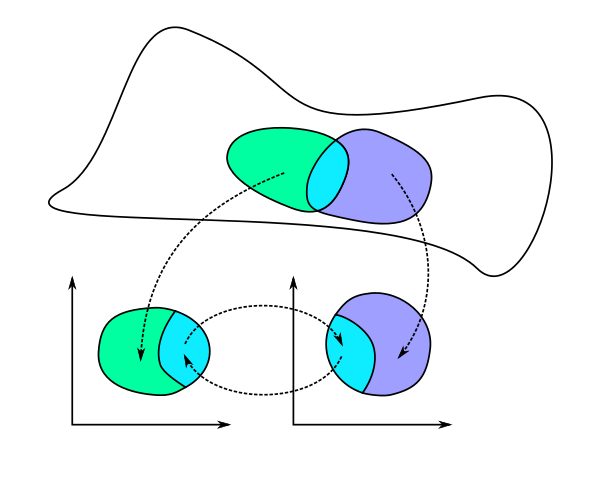
\includegraphics[height=0.25\textheight]{images/manifold} \\
      \tiny a manifold
      \par
    \end{column}
    \begin{column}{0.45\textwidth}
      \centering
      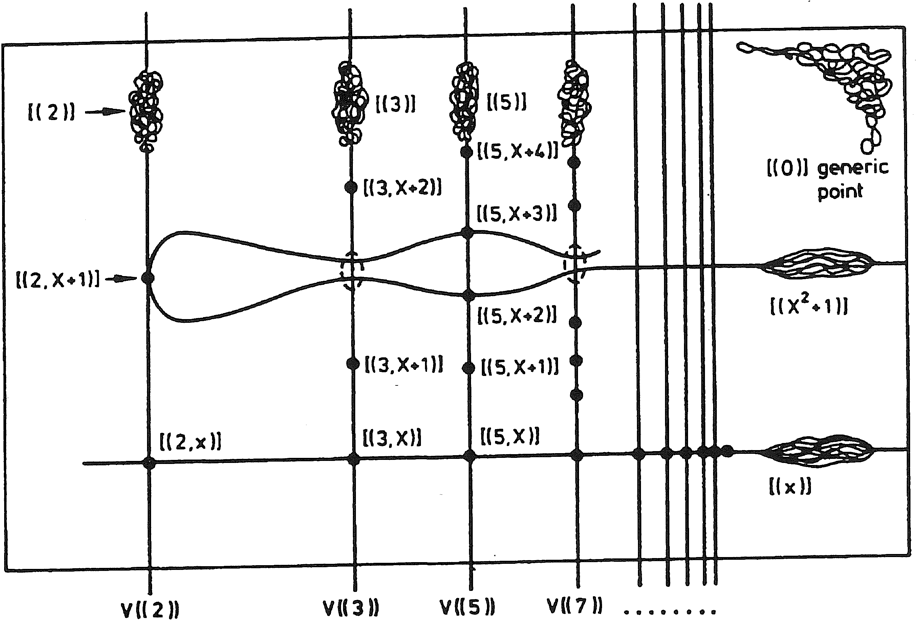
\includegraphics[height=0.25\textheight]{images/mumfords-treasure-map} \\
      \tiny Mumford's treasure map of~$\Spec \ZZ[X]$
      \par
    \end{column}
  \end{columns}
\end{frame}

\note{\justifying
  A \emph{sheaf of rings} on a topological space~$X$ is a ring object
  in~$\Sh(X)$, the category of set-valued sheaves on~$X$.

  A sheaf~$\O_X$ of rings is \emph{local} if and only if all the
  stalks~$\O_{X,x}$ are local rings. Why not demand that the sets of
  sections~$\O_X(U)$ are local rings? This choice has a geometric meaning, but can
  also be motivated from a logical point of view: A sheaf of rings is local if
  and only if, from the point of view of the internal language of~$\Sh(X)$, it
  is a local ring.

  Think of~$\O_X$ as the sheaf of ``number-valued functions'' on~$X$. In
  algebraic geometry, this structure sheaf is a crucial part of the data:
  Wildly different schemes can have the same underlying topological space.
  \par
}

\begin{frame}\frametitle{Motivating the spectrum}
  Let~$A$ be a commutative ring (in~$\Set$).

  Is there a \hil{free local ring}~$A \to A'$ over~$A$?
  \[ \xymatrix{
    A \ar[rd] \ar[rrr] &&& {\substack{\text{local}\\\text{\normalsize$R$}\\\phantom{\text{local}}}} \\
    & {\substack{\text{\normalsize$A'$}\\\text{local}}} \ar@{-->}_[@!34]{\text{local}}[rru]
  } \]

  \hil{No,} if we restrict to~$\Set$.

  \hil{Yes,} if we allow a change of topos:
  Then $A \to \O_{\Spec A}$ is the universal localization.
\end{frame}


\note{\justifying
  Details on this point of view can be found in one of Peter Arndt's very nice
  answers on MathOverflow:
  \begin{center}\url{http://mathoverflow.net/a/14334/31233}\end{center}
  \par
}

\subsection{What is a topos?}

\begin{frame}\frametitle{What is a topos?}
  \begin{block}{Formal definition}A \hil{topos} is a category which has finite limits,
  is cartesian closed and has a subobject classifier.
  \end{block}

  \begin{block}{Motto}A topos is a category which is sufficiently rich to support
  an \hil{internal language}.
  \end{block}

  \begin{block}{Examples}\begin{itemize}
    \item \hil{$\Set$:} \tabto{1.4cm} category of sets
    \item \hil{$\Sh(X)$:} \tabto{1.4cm} category of set-valued sheaves on a space~$X$
  \end{itemize}\end{block}
\end{frame}

\note{\justifying
  While technically correct, the formal definition is actually
  misleading in a sense: A topos has lots of other vital structure, which
  is crucial for a rounded understanding, but is not listed in the
  definition (which is trimmed for minimality).

  A more comprehensive definition is: A \emph{topos} is a locally cartesian
  closed, finitely complete and cocomplete Heyting category which is exact,
  extensive and has a subobject classifier.

  Check out an
  \href{https://ncatlab.org/publications/published/Leinster2011}{article by
  Tom Leinster} for a leisurely introduction to topos theory.
  \par
}


\subsection{What is the internal language?}

\frame[t]{\frametitle{What is the internal language?}
  The internal language of a topos~$\E$ allows to
  \begin{enumerate}
    \item construct objects and morphisms of the topos,
    \item formulate statements about them and
    \item prove such statements
  \end{enumerate}
  in a \hil{naive element-based} language:

  \begin{center}
    \small
    \begin{tabular}{ll}
      \toprule
      externally & internally to $\E$ \\
      \midrule
      object of~$\E$ & set/type \\
      morphism in~$\E$ & map of sets \\
      monomorphism & injective map \\
      epimorphism & surjective map \\
      group object & group \\
      \bottomrule
    \end{tabular}
  \end{center}
}

\frame[t]{\frametitle{The internal language of~$\Sh(X)$}
  \small
  Let~$X$ be a topological space. Then we recursively define
  \[ U \models \varphi \quad \text{(``$\varphi$ holds on~$U$'')} \]
  for open subsets~$U \subseteq X$ and formulas~$\varphi$. Write~``$\Sh(X)
  \models \varphi$'' to mean~$X \models \varphi$.
  \pause
  \[ \renewcommand{\arraystretch}{1.25}\begin{array}{@{}l@{\ }c@{\ }l@{}}
    U \models f = g \? \F &\Ll& f|_U = g|_U \in \F(U) \\
    U \models \varphi \wedge \psi &\Ll&
      \text{$U \models \varphi$ and $U \models \psi$} \\
    U \models \varphi \vee \psi &\Ll&
      \hcancel{\text{$U \models \varphi$ or $U \models \psi$}}{0pt}{3pt}{0pt}{-2pt} \\
    && \text{there exists a covering $U = \bigcup_i U_i$ s.\,th. for all~$i$:} \\
    && \quad\quad \text{$U_i \models \varphi$ or $U_i \models \psi$} \\
    U \models \varphi \Rightarrow \psi &\Ll&
      \text{for all open~$V \subseteq U$: } 
    \text{$V \models \varphi$ implies $V \models \psi$} \\
    U \models \forall f \? \F\_ \varphi(f) &\Ll&
      \text{for all sections~$f \in \F(V), V \subseteq U$: $V \models
      \varphi(f)$} \\
    U \models \exists f \? \F\_ \varphi(f) &\Ll&
      \text{there exists a covering $U = \bigcup_i U_i$ s.\,th. for all~$i$:} \\
    && \quad\quad \text{there exists~$f_i \in \F(U_i)$ s.\,th.
    $U_i \models \varphi(f_i)$}
  \end{array} \]
}

\note{\fontsize{8pt}{9.6}\selectfont
  \begin{itemize}
    \item Special case: The language of~$\Set$ is the usual mathematical language.

    \item \begin{justify}Actually, the objects of~$\E$ feel more like \emph{types} instead of \emph{sets}:
    For instance, there is no global membership relation~$\in$. Rather,
    for each object~$A$ of~$\E$, there is a relation~${\in_A} : A \times \P(A) \to
    \Omega$, where~$\P(A)$ is the power object of~$A$ and~$\Omega$ is the
    object of truth values of~$\E$ (can be understood as the power object of
    a terminal object).\end{justify}

    \item \begin{justify}Compare with the embedding theorem for abelian categories:
    There, an explicit embedding into a category of modules is constructed.
    Here, we only change perspective and talk about the same objects and
    morphisms.\end{justify}

    \item \begin{justify}There exists a weaker variant of the internal language which works
    in abelian categories. By using it, one can even pretend that the objects
    are abelian groups (instead of modules), and when constructing morphisms
    by appealing to the axiom of unique choice (which is a theorem), one
    doesn't even have to check linearity. The proof that this approach
    works uses only categorical logic.\end{justify}

    \item \begin{justify}For expositions of the internal language,
    see Chapters~D1 to~D4 of the Elephant, Chapter~VI of Moerdijk and Mac
    Lane's book, or Chapter~13 of
    \href{http://www.mathematik.tu-darmstadt.de/~streicher/CTCL.pdf}{these
    lecture notes by Thomas Streicher}.\end{justify}
  \end{itemize}
}

\note{\begin{itemize}\justifying
  \item The internal language of a sheaf topos of a $\mathrm{T}_1$-space is
  \emph{classical} (that is, verifies the principle of excluded middle) if and
  only if the space is discrete. That's a not particularly interesting special
  case.
  \item See Section~2.4 of
  \href{https://rawgit.com/iblech/internal-methods/master/notes.pdf}{these
  notes} for remarks on how to appreciate intuitionistic logic.
\end{itemize}}


\note{
  \begin{itemize}
    \item \begin{justify}The rules are called \emph{Kripke--Joyal semantics} and can be
    formulated over any topos (not just sheaf topoi). They are not all
    arbitrary: Rather, they are very finely concerted to make the crucial
    properties about the internal language (see next slide) true.\end{justify}

    \item \begin{justify}If~$\F$ is an object of~$\Sh(X)$, we write
    ``$f:\F$'' instead of~``$f\in\F$'' to remind us that~$\F$ is not really
    (externally) a set consisting of elements, but that we only pretend this
    by using the internal language.\end{justify}

    \item There are two further rules concerning the constants~$\top$
    and~$\bot$ (truth resp. falsehood):
      \[ \renewcommand{\arraystretch}{1.3}\begin{array}{@{}lcl@{}}
        U \models \top &\Ll& U = U \text{ (always fulfiled)}\\
        U \models \bot &\Ll& U = \emptyset
      \end{array} \]

    \item Negation is defined as
    $\neg\varphi :\equiv (\varphi \Rightarrow \bot)$.

    \item \begin{justify}The alternate definition ``$U \models \varphi \vee \psi :\Leftrightarrow
    \text{$U \models \varphi$ or $U \models \psi$}$'' would not be local (cf.
    next slide).\end{justify}
  \end{itemize}
}

\note{
  \begin{itemize}
    \item Let~$\alpha : \F \to \G$ be a morphism of sheaves on~$X$. Then:
    \begin{align*}
      & X \models \speak{$\alpha$ is injective} \\[0.5em]
      \Longleftrightarrow\
      & X \models \forall s,t\?\F\_ \alpha(s) = \alpha(t) \Rightarrow s = t \\[0.5em]
      \Longleftrightarrow\ &
        \text{for all open~$U \subseteq X$, sections $s, t \in \F(U)$:} \\
      &\qquad\qquad
          U \models \alpha(s) = \alpha(t) \Rightarrow s = t \\[0.5em]
      \Longleftrightarrow\ &
        \text{for all open~$U \subseteq X$, sections $s, t \in \F(U)$:} \\
      &\qquad\qquad
          \text{for all open~$V \subseteq U$:} \\
      &\qquad\qquad\qquad\qquad
            \text{$\alpha_V(s|_V) = \alpha_V(t|_V)$ implies $s|_V = t|_V$} \\[0.5em]
      \Longleftrightarrow\ &
        \text{for all open~$U \subseteq X$, sections $s, t \in \F(U)$:} \\
      &\qquad\qquad
            \text{$\alpha_U(s|_U) = \alpha_U(t|_U)$ implies $s|_U = t|_U$} \\[0.5em]
      \Longleftrightarrow\ &
        \text{$\alpha$ is a monomorphism of sheaves}
    \end{align*}

    \item The corner quotes ``$\speak{\ldots}$'' indicate that
    translation into formal language is left to the reader.
  \end{itemize}
}

\note{
  \begin{itemize}
    \item Similarly, we have (exercise, use the rules!):
    \begin{align*}
      &
        X \models \speak{$\alpha$ is surjective} \\[0.5em]
      \Longleftrightarrow\ &
        X \models \forall s\?\G\_ \exists t\?\F\_ \alpha(t) = s \\[0.5em]
      \Longleftrightarrow\ &
        \text{$\alpha$ is an epimorphism of sheaves}
    \end{align*}
  \end{itemize}
}

\note{\fontsize{8pt}{9.6}\selectfont
  \begin{itemize}
    \item One can simplify the rules for often-occuring special cases:
    \[ \renewcommand{\arraystretch}{1.3}\begin{array}{@{}lcl@{}}
      U \models \forall s\?\F\_ \forall t\?\G\_ \varphi(s,t)
      &\Longleftrightarrow&
      \text{for all open~$V \subseteq U$,} \\
      && \text{sections~$s \in \F(V)$, $t \in \G(V)$:} \\
      &&\qquad\qquad V \models \varphi(s,t) \\\\
      U \models \forall s\?\F\_ \varphi(s) \Rightarrow \psi(s)
      &\Longleftrightarrow&
      \text{for all open~$V \subseteq U$, sections~$s \in \F(V)$:} \\
      &&\qquad\qquad \text{$V \models \varphi(s)$ implies $V \models \psi(s)$} \\\\
      U \models \exists!s\?\F\_ \varphi(s)
      &\Longleftrightarrow&
      \text{for all open~$V \subseteq U$,} \\
      &&
      \text{there is exactly one section~$s \in \F(V)$ with:} \\
      &&\qquad\qquad V \models \varphi(s)
    \end{array} \]
  \end{itemize}
}

\note{
  \begin{itemize}
    \item \begin{justify}One can extend the language to allow for \emph{unbounded}
    quantification ($\forall A$ vs.~$\forall a \in A$), by Shulman's
    \emph{stack semantics}. This is needed to formulate
    universal properties internal to~$\Sh(X)$, for instance.\end{justify}

    \item \begin{justify}One can further extend the language to be able to talk
    about locally internal categories over~$\Sh(X)$ (in the sense of
    Penon, see for instance the appendix
    of Johnstone's first topos theory book): Then one can do category theory internal
    to~$\Sh(X)$ using the internal language.

    This specific approach is, as far as I am aware, original work. But of
    course, internal category theory has been done for a long time, see for
    instance the Elephant and also Chapman and Rowbottom's \emph{Relative
    Category Theory and Geometric Morphisms: A Logical Approach}.\end{justify}
  \end{itemize}
}

\frame[t]{\frametitle{The internal language of~$\Sh(X)$}
  \begin{block}{Crucial property: Locality}
    If~$U = \bigcup_i U_i$, then
      $U \models \varphi$ iff $U_i \models
      \varphi$ for all~$i$.
  \end{block}

  \begin{block}{Crucial property: Soundness}
    If~$U \models \varphi$ and $\varphi$
    implies $\psi$ \only<1>{constructively}\only<2->{\pointthis{constructively}{
      no $\varphi \vee \neg\varphi$,\ \
      no $\neg\neg\varphi \Rightarrow \varphi$,\ \
      no AxC
    }},
    then~$U \models \psi$.
  \end{block}

  \vfill

  \pause\pause
  \begin{block}{A first glance at the constructive nature}
  \begin{itemize}
    \item $U \models f = 0$
      \tabto{2.75cm} iff $f|_U = 0 \in \F(U)$.
    \item $U \models \neg\neg(f = 0)$
      \tabto{2.75cm} iff~$f = 0$ on a dense open subset of~$U$.
  \end{itemize}
  \end{block}
}

\note{\scriptsize%
  \vspace{-0.5em}%
  \begin{center}\large\bf Why is constructive mathematics
  interesting?\end{center}
  \vspace{-1em}
  \begin{itemize}
    \item The internal logic of most toposes is constructive.

    \item \begin{justify}From a constructive proof of a statement, it's always possible to
    mechanically extract an \emph{algorithm} witnessing its truth. For example:
    A proof of the infinitude of primes gives rise to an algorithm
    which actually computes infinitely many primes (outputting one at a
    time, never stopping).\end{justify}

    \item \begin{justify}By the celebrated \emph{Curry--Howard correspondence},
    constructive truth of a formula is equivalent to the existence of a
    program of a certain type associated to the formula.\end{justify}

    \item \begin{justify}In constructive mathematics, one can experiment with (and draw
    useful conclusions also holding in a usual sense) \emph{anti-classical
    dream axioms}, for instance the one of synthetic differential geometry:\end{justify}
    \begin{quote}All functions~$\RR \to \RR$ are smooth.\end{quote}

    \item \begin{justify}Constructive accounts of classical theories are sometimes more
    elegant or point out some minor but interesting points which are not appreciated by a
    classical perspective.\end{justify}

    \item \begin{justify}The philosophical question on the \emph{meaning of truth} is
    easier to tackle in constructive mathematics.\end{justify}
  \end{itemize}
}

\note{\scriptsize%
  \vspace{-0.5em}%
  \begin{center}\large\bf Three rumours about constructive mathematics\end{center}
  \vspace{-1em}

  \begin{enumerate}
    \item \begin{justify}There is a false rumour about constructive mathematics, namely that
    the term \emph{contradiction} is generally forbidden. This is not the
    case, one has to distinguish between
    \begin{itemize}
      \item\scriptsize a true proof by contradiction: ``Assume~$\varphi$ were false.
      Then \ldots, contradiction. So~$\varphi$ is in fact true.''
    \end{itemize}
    which constructively is only a proof of the weaker
    statement~$\neg\neg\varphi$, and
    \begin{itemize}
      \item\scriptsize a proof of a negated formula: ``Assume~$\psi$ were true. Then
      \ldots, contradiction. So~$\neg\psi$ holds.''
    \end{itemize}
    which is a perfectly fine proof of~$\neg\psi$ in constructive mathematics.\end{justify}

    \item \begin{justify}There is a similar rumour that constructive mathematicians \emph{deny}
    the law of excluded middle. In fact, one can constructively prove that there is no
    counterexample to the law: For any formula~$\varphi$, it holds
    that~$\neg\neg(\varphi \vee \neg\varphi)$.

    In constructive mathematics, one merely doesn't \emph{use} the law of
    excluded middle. (Only in concrete models, for example as provided by the
    internal universe of the sheaf topos on a non-discrete topological space,
    the law of excluded middle will actually be refutable.)\end{justify}
  \end{enumerate}
}

\note{
  \begin{enumerate}
    \item[3.]\scriptsize \begin{justify}There is one last false rumour about constructive mathematics: Namely
    that most of mathematics breaks down in a constructive setting. This is
    only true if interpreted naively: Often, already very small changes to the
    definitions and statements (which are classically simply equivalent
    reformulations) suffice to make them constructively acceptable.

    In other cases, adding an additional hypothesis, which is classically
    always satisfied, is necessary (and interesting). Here is an example: In
    constructive mathematics, one can not show that any inhabited subset of the
    natural numbers possesses a minimal element. [One can also not show the
    negation -- recall the previous false rumour.] But one can show (quite
    easily, by induction) that any inhabited and \emph{detachable} subset
    of the natural numbers possesses a minimal element. A subset~$U \subseteq
    \NN$ is detachable iff for any number~$n \in \NN$, it holds that~$n
    \in U$ or~$n \not\in U$.

    This has a computational interpretation: Given an arbitrary inhabited subset~$U
    \subseteq \NN$, one cannot algorithmically find its minimal element. But it
    \emph{is} possible if one has an algorithmic \emph{test of membership}
    for~$U$.\end{justify}
  \end{enumerate}

  \begin{justify}\scriptsize References about constructive mathematics include:
  \begin{itemize}
  \item Bridges. Constructive Mathematics.
  \item van Dalen. Intuitionistic logic.
  \item Troelstra and van Dalen. Constructivism in Mathematics: An Introduction.
  \end{itemize}
  \href{http://math.andrej.com/category/constructive-math/}{Andrej Bauer's
  blog} is also very informative.\end{justify}
}


\section{The little Zariski topos of a scheme}
\subsection{Basic look and feel}

\frame[t]{\frametitle{The little Zariski topos}
  \begin{block}{Definition}The \hil{little Zariski topos} of a scheme~$X$ is the
  category~$\Sh(X)$ of set-valued sheaves on~$X$.\end{block}

  \begin{block}{Basic look and feel}
  \begin{itemize}
    \item Internally, the structure sheaf~$\O_X$ looks like \[ \text{
    an ordinary ring.} \]
    \item Internally, a sheaf of~$\O_X$-modules looks like \[
    \text{an ordinary module on that ring.} \]
  \end{itemize}
  \end{block}
}


\subsection{Building and using a dictionary}

\begin{frame}\frametitle{Building a dictionary}
  \sloganwithoutborder{\hil{Understand notions of algebraic geometry
  as notions of algebra internal to~$\boldsymbol{\Sh(X)}$.}}
  \begin{center}
    \small
    \scalebox{0.93}{\begin{tabular}{ll}
      \toprule
      externally & internally to $\Sh(X)$ \\
      \midrule
      sheaf of sets & set/type \\
      morphism of sheaves & map of sets \\
      monomorphism & injective map \\
      epimorphism & surjective map \\
      \midrule
      sheaf of rings & ring \\
      sheaf of modules & module \\
      sheaf of finite type & finitely generated module \\
      finite locally free sheaf & finite free module \\
      % coherent sheaf & coherent module \\
      tensor product of sheaves & tensor product of modules \\
      % sheaf of rational functions & total quotient ring of~$\O_X$ \\
      sheaf of Kähler differentials & module of Kähler differentials \\
      sheaf of rational functions & total quotient ring of~$\O_X$ \\
      dimension of $X$ & Krull dimension of~$\O_X$ \\
      \bottomrule
    \end{tabular}}
  \end{center}

  \visible<2>{\begin{tikzpicture}[overlay]
    \draw[fill=white, draw=white, opacity=0.9] (0,0) rectangle (\paperwidth,6.6);
    \node[anchor=south west,inner sep=0] (image) at (1.8,1.3) {
      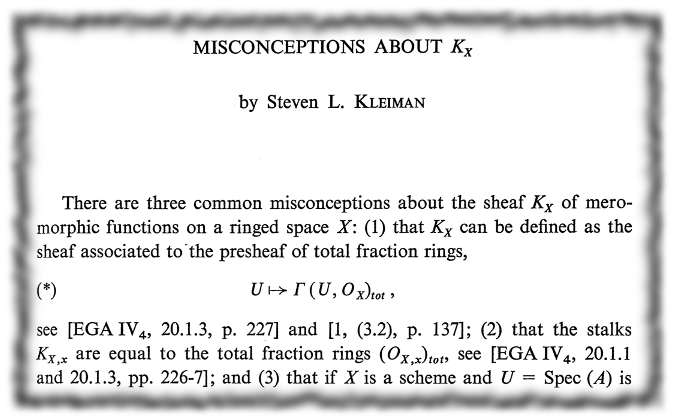
\includegraphics[width=0.7\textwidth]{images/steven-kleiman-misconceptions-about-kx}
    };
  \end{tikzpicture}}
\end{frame}

\note{\justifying
  See the \href{https://rawgit.com/iblech/internal-methods/master/notes.pdf}{notes} for more dictionary entries.

  The simple definition of~$\K_X$ allows to give an internal account of the
  basics of the theory of Cartier divisors, for instance giving an easy
  description of the line bundle associated to a Cartier divisor.
  \par
}

\begin{frame}\frametitle{Using the dictionary}
  \begin{center}
    \begin{minipage}{0.70\textwidth}
      \begin{exampleblock}{}
        \justifying
        Let~$0 \to M' \to M \to M'' \to 0$ be a short exact sequence of
        modules. If~$M'$ and~$M''$ are finitely generated, so is~$M$.
      \end{exampleblock}
    \end{minipage}
    \medskip

    \scalebox{3}{$\Downarrow$}

    \begin{minipage}{0.70\textwidth}
      \begin{exampleblock}{}
        \justifying
        Let $0 \to \F' \to \F \to \F'' \to 0$ be a short exact sequence
        of sheaves of~$\O_X$-modules. If~$\F'$ and~$\F''$ are of finite type,
        so is~$\F$.
      \end{exampleblock}
    \end{minipage}
  \end{center}
\end{frame}

\begin{frame}[c]\frametitle{Using the dictionary}
  \begin{center}
    \begin{minipage}{0.70\textwidth}
      \begin{exampleblock}{}
        \justifying
        Any finitely generated vector space does \emph{not not} possess a basis.
      \end{exampleblock}
    \end{minipage}
    \medskip

    \scalebox{3}{$\Downarrow$}

    \begin{minipage}{0.70\textwidth}
      \begin{exampleblock}{}
        \justifying
        Any sheaf of modules of finite type on a reduced scheme is locally free
        \emph{on a dense open subset}.
      \end{exampleblock}
      \centering
      \tiny Ravi Vakil: ``Important hard exercise'' (13.7.K).
      \par
    \end{minipage}
  \end{center}
\end{frame}

\begin{frame}\frametitle{The objective}
  \slogan{\justifying Understand notions and statements of \hil{algebraic geometry} as
  notions and statements of (intuitionistic) \hil{commutative
  algebra} internal to suitable \hil{toposes}.}

%  In order to:
%  \begin{itemize}
%    \item Gain conceptual understanding.
%    \item Simplify proofs.
%    \item Develop a synthetic account of scheme theory.
%    \item Contribute to constructive algebra.
%  \end{itemize}

  Further topics in the little Zariski topos:
  \begin{itemize}
    \item Upper semicontinuous rank function
    \item Transfer principles~$M \leftrightarrow M^\sim$
    \item The curious role of affine open subsets
    \item Quasicoherence
    \item Spreading from points to neighbourhoods
    \item The relative spectrum
  \end{itemize}
\end{frame}

\begin{frame}[c]\frametitle{Praise for Mike Shulman}
  \centering
  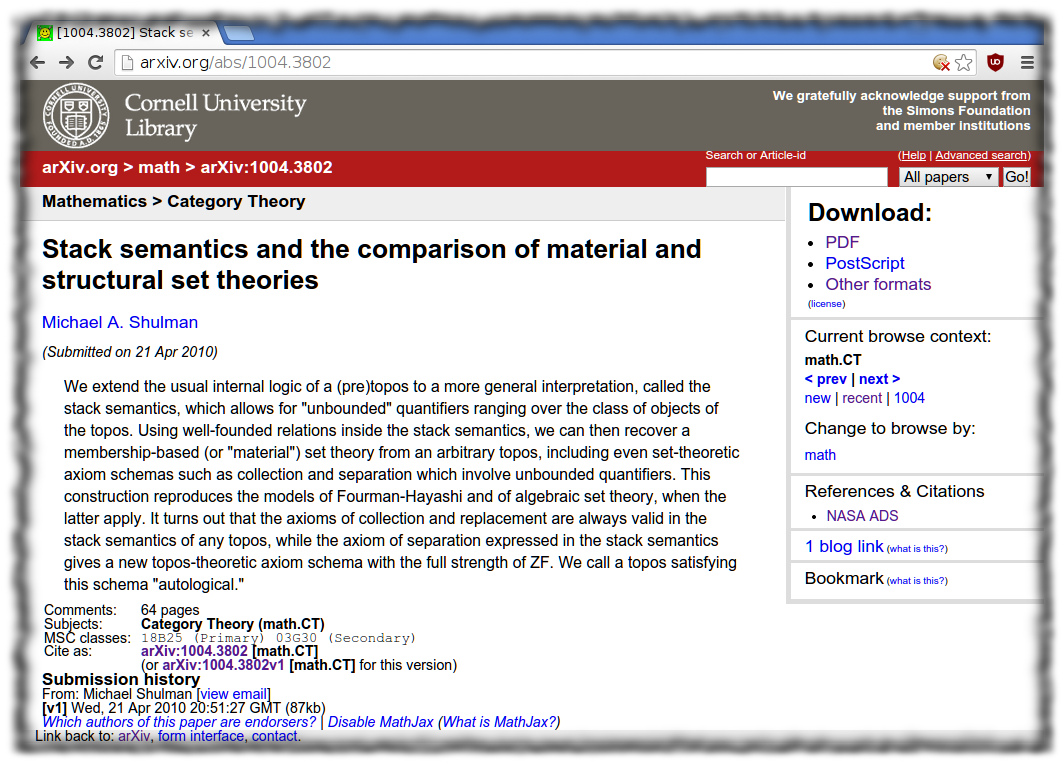
\includegraphics[scale=0.4]{images/mike-shulman-stack-semantics}
  \par
\end{frame}

\note{\justifying
  The internal language of a topos supports
  \begin{itemize}
  \item first-order logic,
  \item higher-order logic (for instance quantification over subsets),
  \item dependent types, and
  \item unbounded quantification.
  \end{itemize}

  The first three items are standard. The fourth is due to Mike Shulman.
  Combined, it's possible to interpret ``essentially all of constructive
  mathematics'' internal to a topos.

  Restrictions persist for operations with a ``set-theoretical flavor'' like
  building an infinite union of iterated powersets, for example~$\bigcup_{n \in
  \NN} P^n(\NN)$.
  \par
}


\subsection{The rank function of sheaves of modules}

\begin{frame}\frametitle{The rank function of sheaves of modules}
  There is the following one-to-one correspondence:
  \[\small
    \underunbrace{\fmini{0.35\textwidth}{upper semi-continuous \\ functions on~$X$}}_{\text{external}}
    \xleftrightarrow{\quad\text{1:1}\quad}
    \underunbrace{\fmini{0.4\textwidth}{completed natural numbers}}_{\text{internal}}
  \]

  \vfill

  \begin{center}
    \small
    \begin{minipage}{0.42\textwidth}
      \begin{exampleblock}{}
        \justifying
        Let~$M$ be a f.\,g.\@ $A$-module. Assume that $A$ is a field.
        Then~$M$ is free iff the minimal number of generators is an
        actual natural number.
      \end{exampleblock}
    \end{minipage}
    \quad\scalebox{3}{$\Rightarrow$}\quad
    \begin{minipage}{0.37\textwidth}
      \begin{exampleblock}{}
        \justifying
        Let~$\F$ be an~$\O_X$-module of finite type. Assume that~$X$ is reduced.
        Then~$\F$ is locally free iff its rank is locally constant.
      \end{exampleblock}
    \end{minipage}
  \end{center}
\end{frame}

\note{
  \begin{block}{Proposition}
    If every inhabited subset of the natural numbers has a minimum, then the
    law of excluded middle holds. (So in constructive mathematics, one cannot
    prove the natural numbers to be complete in this sense.)
  \end{block}

  \begin{block}{Proof}
    Let~$\varphi$ be an arbitrary formula. Define the subset
    \[ U \defeq \{ n \in \NN \,|\, n = 1 \vee \varphi \} \subseteq \NN, \]
    which surely is inhabited by~$1 \in U$. So by assumption, there exists a
    number~$z \in \NN$ which is the minimum of~$U$. We have
    \[ z = 0 \quad\vee\quad z > 0 \]
    (this is constructively not trivial, but can be proven by induction).

    If~$z = 0$, we have~$0 \in U$, so~$0 = 1 \vee \varphi$, so~$\varphi$
    holds.

    If~$z > 0$, then~$\neg\varphi$ holds: Because if~$\varphi$ were
    true, zero would be an element of~$U$, contradicting the minimality of~$z$.
  \end{block}
}

\note{
  \begin{block}{Proposition}
    The partially ordered set
    \[ \widehat\NN \defeq \{ A \subseteq \NN \,|\, \text{$A$ inhabited and upward
    closed}
    \} \]
    is the least partially ordered set containing~$\NN$ and possessing minima
    of arbitrary inhabited subsets.
  \end{block}

  The embedding $\NN \hookrightarrow \widehat\NN$ is given by
  \[ n \in \NN \longmapsto {\uparrow}(n) \defeq \{ m \in \NN \,|\, m \geq n \}. \]

  \begin{block}{Proof}
    If~$M \subseteq \widehat\NN$ is an inhabited subset, its minimum is
    \[ \min M = \bigcup M \in \widehat\NN. \]
    The proof of the universal property is straightforward.
  \end{block}
}

\note{
  \begin{block}{External translation (see Mulvey's \emph{Intuitionistic algebra
  and representations of rings})}
    Let~$X$ be a topological space and consider the constant sheaf~$N$ with
    $\Gamma(U, N) = \{ f : U \to \NN \,|\ \text{$f$ continuous} \}$.
    Internally, the sheaf~$N$ plays the role of the ordinary natural numbers.
    Then there is an one-to-one correspondence:
    \begin{enumerate}
      \item Let~$A \hookrightarrow N$ be a subobject which is inhabited
      and upward closed from the internal point of view. Then
      \[
        x \longmapsto \inf\{ n \in \NN \,|\, n \in A_x \}
      \]
      is an upper semi-continuous function on~$X$.

      \item Let~$\alpha : X \to \NN$ be a upper semi-continuous function. Then
      \[ U \subseteq X \longmapsto \{ f : U \to \NN \,|\, \text{$f$
      continuous,\ \ $f \geq \alpha$ on~$U$} \} \]
      is a subobject of~$N$ which internally is inhabited and upward closed.
    \end{enumerate}
  \end{block}

  Under the correspondence, locally \emph{constant}
  functions map exactly to the [image of the] \emph{ordinary} internal natural numbers
  [in the completed natural numbers].
}

\note{
  \begin{itemize}
    \item Here is an explicit example of a completed natural number which is
    not an ordinary natural number: Let~$X =
    \Spec k[X]$ and~$\F = k[X]/(X-a)^\sim$. The rank of~$\F$ is~$1$ at~$a$ and
    zero elsewhere. It corresponds to the internal completed natural number
    \begin{multline*}
      z \defeq \min \{ n \in \NN \,|\, \speak{$\F$ can be generated by~$n$ elements} \} = \\
        \min\{ n \in \NN \,|\, n \geq 1 \vee \speak{the element $(X-a)$ of~$\O_X$
        is invertible} \}.
    \end{multline*}
    We have the internal implications
    \begin{align*}
      \Sh(X) \models \phantom{\neg}\,\speak{$(X-a)$ inv.} \Rightarrow z = 0\phantom{,} \\
      \Sh(X) \models \neg\,\speak{$(X-a)$ inv.} \Rightarrow z = 1,
    \end{align*}
    but we do \emph{not} have
    \begin{align*}
      \Sh(X) \models \speak{$(X-a)$ inv.} \ \vee\ \neg\,\speak{$(X-a)$ inv.},
    \end{align*}
    which would imply
    \begin{align*}
      \Sh(X) \models z = 0 \vee z = 1,
    \end{align*}
    i.\,e. the false statement that~$\F$ is locally free (of ranks~$0$ resp.~$1$).
  \end{itemize}
}

\note{
  \begin{itemize}
    \item \begin{justify}Here is a constructive proof of the statement that
    finitely generated vector spaces, for which the minimal number of
    generators is an actual natural numbers, are free:

    By assumption, the minimal number~$n \in \NN$ of generators for~$M$ exists.
    Let~$x_1,\ldots,x_n$ be a generating family of minimal length~$n$. We want
    to verify that it's linearly independent, so that it constitutes a basis.

    Let~$\sum_i \lambda_i x_i = 0$. If any~$\lambda_i$
    were invertible, the shortened family $x_1,\ldots,x_{i-1},$ $x_{i+1},\ldots,x_n$
    would also generate~$M$. By minimality of~$n$, this is not possible. So
    each~$\lambda_i$ is not invertible. By the field assumption on~$A$, it
    follows that each~$\lambda_i$ is zero.\end{justify}

    \item \begin{justify}In constructive mathematics, one can not show that
    every finitely generated vector space over a field admits a finite basis.
    (Exercise: Prove this by showing that this would imply the law of excluded
    middle.)
    This is not because the space might strangely turn out to be
    infinite-dimensional, but merely because one may not be able to explicitly
    exhibit a finite basis.\end{justify}
  \end{itemize}
}


\subsection{Transfer principles}

\begin{frame}\frametitle{Transfer principles}

  \hil{Question:} How do the properties of
  \begin{itemize}
  \item an~$A$-module~$M$ in~$\Set$ and
  \item the~$\O_X$-\only<2->{module}\only<1>{\pointthis{module}{an important
  sheaf with~$M^\sim(X) = M$}}~$M^\sim$ in~$\Sh(X)$, where~$X = \Spec A$, relate?
  \end{itemize}
  \pause
  \vfill

  \hil{Observation:} $M^\sim = \underline{M}[\F^{-1}]$, where
  \begin{itemize}
  \item $\underline{M}$ is the constant sheaf with stalks~$M$ on~$X$ and
  \item $\F \hookrightarrow \underline{A}$ is the \hil{generic prime filter}.
  \end{itemize}
  Note: $M$ and $\underline{M}$ share all first-order properties.
  \pause
  \vfill

  \centering
  \hil{Answer:} $M^\sim$ inherits those properties of $M$ which are \\
  \hil{stable under localization}.
  \par
\end{frame}

\note{\justifying
  The concept of a \emph{prime filter} is a direct axiomatization of what you
  expect the complement of a prime ideal to fulfil. In classical logic,
  complementation gives a bijection between the prime filters and the prime
  ideals of a ring.

  Prime filters are important in constructive mathematics because localizing
  them gives rise to local rings. In contrast, localizing a ring at the
  complement of a prime ideal doesn't usually result in a local ring.

  To construct the universal localization of~$A$, one doesn't pick a particular
  prime filter~$F$ to construct~$A[F^{-1}]$. Instead, one picks the
  \emph{generic prime filter}~$\F$. This filter doesn't live in~$\Set$, but
  in~$\Sh(\Spec A)$.
  \par
}


\subsection{The curious role of affine open subsets}

\begin{frame}\frametitle{The curious role of affine open subsets}
  \hil{Question:} Why do the following identities hold, for quasicoherent
  sheaves~$\E$ and~$\F$ and affine open subsets~$U$?
  \begin{align*}
    (\E/\F)(U) &= \E(U) / \F(U) \\
    (\E \otimes_{\O_X} \F)(U) &= \E(U) \otimes_{\O_X(U)} \F(U) \\
    \E_\mathrm{tors}(U) &= \E(U)_\mathrm{tors} \quad\text{(sometimes)} \\
    \K_X(U) &= \operatorname{Quot} \O_X(U) \quad\text{(sometimes)}
  \end{align*}
  \pause
  \hil{A calculation:}
  \begin{align*}
    M^\sim \otimes_{\O_U} N^\sim &=
    \ull{M}[\F^{-1}] \otimes_{\ull{A}[\F^{-1}]} \ull{N}[\F^{-1}] =
    (\ull{M} \otimes_\ull{A} \ull{N})[\F^{-1}] \\
    &= (\ull{M \otimes_A N})[\F^{-1}] =
    (M \otimes_A N)^\sim.
  \end{align*}
  \pause
  \hil{Answer:} Because localization commutes with quotients, tensor products,
  torsion submodules (sometimes), \ldots
\end{frame}


\subsection{Quasicoherence of sheaves of modules}

\begin{frame}\frametitle{A curious property of the structure sheaf}
  Let~$X$ be a scheme. Internally to~$\Sh(X)$,
  \begin{center}
    \hil{any non-invertible element of~$\boldsymbol{\O_X}$ is nilpotent.}
  \end{center}

  \centering
  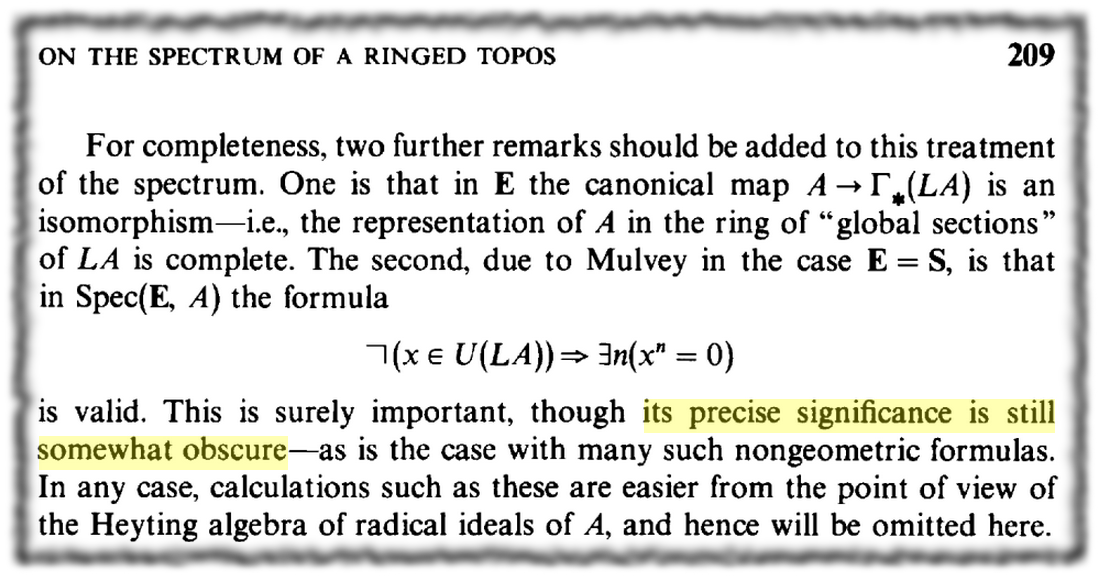
\includegraphics[scale=0.3]{images/tierney-on-the-spectrum-of-a-ringed-topos} \\
  \tiny
  %Miles Tierney. ``On the spectrum of a ringed topos''. \\ In: \emph{Algebra,
  %Topology, and Category Theory. A Collection of Papers in Honor of Samuel
  %Eilenberg}. Ed.\@ by A.~Heller and M.~Tierney. Academic Press, 1976,
  %pp.~189--210.
  Miles Tierney. On the spectrum of a ringed topos. 1976.
  \par
\end{frame}

\begin{frame}\frametitle{Quasicoherence}
  Let~$X$ be a scheme. Let~$\E$ be an~$\O_X$-module.

  Then~$\E$ is quasicoherent
  if and only if, internally to~$\Sh(X)$,
  \begin{quote}\textnormal{$\E[f^{-1}]$ is a $\Box_f$-sheaf for any~$f : \O_X$, \\[0.3em]
  \qquad\qquad where~$\Box_f\varphi \defeqv (\text{$f$ invertible} \Rightarrow \varphi)$.}
  \end{quote}
  \pause

  In particular: If~$\E$ is quasicoherent, then internally
  \[ (\text{$f$ invertible} \Rightarrow s = 0) \Longrightarrow
    \bigvee_{n \geq 0} f^n s = 0 \]
  \vspace*{-1.5em}\par%
  for any~$f : \O_X$ and~$s : \E$.
\end{frame}

\note{\justifying
  The sheaf condition and the sheafification functor can be described purely
  internally. An object~$M$ is \emph{separated} with respect to~$\Box$ if
  and only if, from the internal point of view,
  \[ \forall x,y : M\_\ \Box(x = y) \Rightarrow x = y. \]
  It is a \emph{sheaf} with respect to~$\Box$, if furthermore
  \[ \forall K \subseteq M\_\
    \Box(\exists x : M\_\ K = \{ x \}) \Longrightarrow
    \exists x : M\_\ \Box(x \in K). \]

  The second condition displayed on the previous slide is equivalent to the
  separatedness condition. In the special case~$\E = \O_X$, $s = 1$ it reduces
  to Mulvey's ``somewhat obscure formula''. We now understand this condition in
  its proper context.
  \par
}


\subsection{Spreading of properties}

\newcommand{\idiamond}{{\usebeamercolor[fg]{item}{\boldsymbol{\Box}}}}
\newcommand{\gdiamond}[1]{\textcolor{gray}{\boldsymbol{\Box}(}#1\textcolor{gray}{)}}

\begin{frame}\frametitle{The $\Box$-translation}
  Let~$\E_\Box \hookrightarrow \E$ be a subtopos given by a local
  operator. Then
  \[ \E_\Box \models \varphi \qquad\text{iff}\qquad
    \E \models \varphi^\Box\only<2->{.}\only<1>{,}\]
  \only<1>{where the translation~$\varphi \mapsto \varphi^\Box$ is given by:
  \begin{align*}
    (s = t)^\Box &\defeqv \idiamond(s=t) \\
    (\varphi \wedge \psi)^\Box &\defeqv \gdiamond{\varphi^\Box \wedge \psi^\Box} \\
    (\varphi \vee \psi)^\Box &\defeqv \idiamond(\varphi^\Box \vee \psi^\Box) \\
    (\varphi \Rightarrow \psi)^\Box &\defeqv \gdiamond{\varphi^\Box \Rightarrow \psi^\Box} \\
    (\forall x\?X\_ \varphi(x))^\Box &\defeqv \gdiamond{\forall x\?X\_ \varphi^\Box(x)} \\
    (\exists x\?X\_ \varphi(x))^\Box &\defeqv \idiamond(\exists x\?X\_ \varphi^\Box(x))
  \end{align*}}%
  \only<2->{%
    Let~$X$ be a scheme. Depending on~$\Box$,~$\Sh(X)
    \models \Box\varphi$ means that~$\varphi$ holds on \ldots
    \begin{itemize}
      \item \ldots{} a dense open subset.
      \item \ldots{} a schematically dense open subset.
      \item \ldots{} a given open subset~$U$.
      \item \ldots{} an open subset containing a given closed subset~$A$.
      \item \ldots{} an open neighbourhood of a given point~$x \in X$.
    \end{itemize}

    \pause
    Can tackle the question~``$\varphi^\Box \stackrel{?}{\Rightarrow} \Box\varphi$'' logically.
  }
\end{frame}

\note{\justifying
  The~$\Box$-translation is a generalization of the \emph{double negation
  translation}, which is well-known in logic. The double negation translation
  has the following curious property: A formula~$\varphi$ admits a classical
  proof if and only if the translated formula~$\varphi^{\neg\neg}$ admits an
  intuitionistic proof.

  The~$\Box$-translation has been studied before (see for instance Aczel:
  \emph{The Russell--Prawitz modality}, and Escardó, Oliva: \emph{The Peirce
  translation and the double negation shift}), but to the best of my know\-ledge,
  this application -- expressing the internal language of
  subtoposes in the internal language of the ambient topos -- is new.
  \par
}

\note{\justifying
  For ease of exposition, assume that~$X$ is irreducible with generic
  point~$\xi$. Let~$\Box \defeqv \neg\neg$.

  Then~$\Sh(X) \models \Box \varphi$ means that~$\varphi$ holds on a dense
  open subset of~$X$, while~$\Sh(X) \models \varphi^\Box$ means
  that~$\varphi$ holds at the generic point (taking stalks of all involved
  sheaves).

  The question~``does~$\varphi^\Box$ imply~$\Box\varphi$?'' therefore
  means: Does~$\varphi$ spread from the generic point to a dense open subset?

  For the special case of the double negation translation, a general answer to
  this purely logical question has long been known: This holds if~$\varphi$ is
  a \emph{geometric formula} (doesn't contain~$\Rightarrow$ and~$\forall$).
  \par
}

\note{\justifying
  Let~$\F$ be a sheaf of modules on a locally ringed space~$X$.
  Assume that the stalk~$\F_x$ at some point~$x \in X$ vanishes.
  Then in general it does \emph{not} follow that~$\F$ vanishes on some open
  neighbourhood of~$x$.

  This can be understood in logical terms: The statement that~$\F$ vanishes,
  \[ \forall s : \F\_\ s = 0, \]
  is not a geometric formula.

  However, if~$\F$ is additionally supposed to be of finite type, then it
  \emph{does} follow that~$\F$ vanishes on an open neighbourhood. This too can
  be understood in logical terms: If~$\F$ is of finite type, then internally
  there are generators~$s_1,\ldots,s_n$ of~$\F$. Thus the vanishing of~$\F$ can
  be reformulated as
  \[ s_1 = 0 \wedge \cdots \wedge s_n = 0, \]
  and this condition is manifestly geometric.
  \par
}


\subsection{The relative spectrum}

\newcommand{\defspeca}{\text{topological space of the prime ideals of $A$}}
\newcommand{\defspecb}{\text{topological space of the prime filters of $A$}}
\newcommand{\defspecc}{\text{locale of the prime filters of $A$}}

\begin{frame}\frametitle{The absolute spectrum, internalised}
  Let~$A$ be a commutative ring in a topos~$\E$.

  To construct the \hil{free local ring} over~$A$, give a constructive account
  of the spectrum:
  \begin{align*}
    \only<1>{\Spec A &\defeq \defspeca}
    \only<2->{\Spec A &\defeq \hcancel{$\defspeca$}{0pt}{3pt}{0pt}{-2pt}}
    \\
    \only<3>{&\defeq \defspecb}
    \only<4->{&\defeq \hcancel{$\defspecb$}{0pt}{3pt}{0pt}{-2pt}}
    \\
    \only<5->{&\defeq \defspecc}
  \end{align*}
  \pause
  \pause
  \pause
  \pause
  The frame of opens of~$\Spec A$ is the frame of radical ideals
  in~$A$. Universal property:
  \[ \Hom_{\mathrm{LRT}/|\E|}(T, \Spec A) \cong \Hom_{\mathrm{Ring}(\E)}(A, \mu_*\O_T) \]
  for all locally ringed toposes~$T$ equipped with a geometric morphism~$T \xrightarrow{\mu} \E$.
\end{frame}

\note{\justifying
  The axioms of a prime filter constitute a propositional geometric theory.
  Therefore there exists the \emph{classifying locale} over prime filters. This
  is the ring's spectrum. See Vicker's
  \href{http://www.cs.bham.ac.uk/~sjv/LocTopSpaces.pdf}{Locales and Toposes as Spaces} and
  \href{http://www.cs.bham.ac.uk/~sjv/GeoAspects.pdf}{Continuity and geometric
  logic} for very accessible introductions to this topic.

  Monique Hakim constructed in her thesis a very general spectrum functor,
  taking a ringed topos to a locally ringed one, using explicit calculations
  with sites.

  Using the internal language allows to reduce these calculations to a minimum.
  One constructs the spectrum as the sheaf topos over an internal
  locale and then uses the general theorem that toposes over the base~$\E$ are
  the same as toposes internal to~$\E$.

  As a byproduct one obtains that Hakim's spectrum is \emph{localic} over the base.
  \par
}

\begin{frame}\frametitle{The relative spectrum}
  Let~$X$ be a scheme and~$\A$ be a quasicoherent~$\O_X$-algebra.
  Can we describe its \hil{relative spectrum}~$\RelSpec_X \A \to X$ internally?

  Desired universal property:
  \[ \Hom_{\mathrm{LRL}/X}(T, \RelSpec_X \A) \cong \Hom_{\mathrm{Alg}(\O_X)}(\A,
  \mu_*\O_T) \]
  for all locally ringed locales~$T$ over~$X$.
  \pause

  \only<2>{\begin{exampleblock}{Beware of believing false statements}
  \begin{itemize}
  \item $\RelSpec_X \O_X = X$.
  \item $\Spec \A$ is the one-point locale iff every element
  of~$\A$ is invertible or nilpotent.
  \item Every element of~$\O_X$ which is not invertible is nilpotent.
  \item Thus cannot prove~$\Spec \O_X = \mathrm{pt}$ internally.
  \end{itemize}\end{exampleblock}}
  \pause

  \hil{Solution:} Define internally the frame of~$\RelSpec_X \A$ to be the frame of
  those radical ideals~$I \subseteq \A$ such that
  \[ \forall f\?\O_X\_ \forall s\?\A\_
    (\text{$f$ invertible in~$\O_X$} \Rightarrow s \in I) \Longrightarrow
      fs \in I. \]
  \pause
  Its \hil{points} are those prime filters~$G$ of~$\A$ such that
  \[ \forall f\?\O_X\_ \varphi(f) \in G \Longrightarrow \text{$f$ invertible in~$\O_X$}. \]
\end{frame}

\note{\justifying
  The stated condition on~$I$ is, under the assumption that~$\A$ is
  quasicoherent, equivalent to the condition that~$I$ is quasicoherent (as
  an~$\O_X$-module).

  The relative spectrum is thus constructed as a certain sublocale of the
  absolute one. The two constructions coincide if and only if the dimension of
  the base scheme is~$\leq 0$.

  If~$X$ is not a scheme or~$\A$ is not quasicoherent, the construction still
  gives rise to a locally ringed locale over~$X$ which satisfies the universal
  property
  \[ \Hom_{\mathrm{LRL}/X}(T, \RelSpec_X \A) \cong \Hom_{\mathrm{Alg}(\O_X)}(\A,
  \mu_*\O_T) \]
  for all locally ringed locales~$T \xrightarrow{\mu} X$ over~$X$.
  \par
}

\begin{frame}\frametitle{The relative spectrum, reformulated}
  Let~$B \to A$ be an algebra in a topos.

  Is there a \hil{free local and local-over-$\boldsymbol{B}$ ring}~$A \to A'$ over~$A$?

  \[ \xymatrix{
    B \ar[r]\ar@/^2pc/[rrrr]^{\text{local}}\ar@/_/[rrd]_[@!-33]{\text{local}} &
      A \ar[rd] \ar[rrr] &&&
      {\substack{\text{local}\\\text{\normalsize$R$}\\\phantom{\text{local}}}} \\
    && {\substack{\text{\normalsize$A'$}\\\text{local}}} \ar@{-->}[rru]_[@!35]{\text{local}}
  } \]

  \medskip
  Form limits in the category of \hil{locally ringed locales}
  by \hil{relocalizing} the corresponding limit in ringed locales.
\end{frame}

\note{\justifying
  One might wonder whether the absolute spectrum or the relative one is ``more
  fundamental''. The absolute spectrum can be expressed using the relative one,
  since
  \[ \Spec A = \RelSpec_{\Spec \ZZ} A^{\sim}, \]
  but the other way is not in general possible: The absolute spectrum is always
  (quasi-)compact, while the relative one is not in general.
  \par
}
% XXX: Give details.


\section{The big Zariski topos of a scheme}

\subsection{Basic look and feel}

\begin{frame}\frametitle{The big Zariski topos}
  \begin{block}{Definition}The \hil{big Zariski topos} $\Zar(S)$ of a scheme~$S$ is the
  category $\Sh(\Sch/S)$. It consists of certain functors
  $(\Sch/S)^\op \to \Set$.
  \end{block}

  \begin{block}{Basic look and feel}
  \begin{itemize}
    \item For an~$S$-scheme~$X$, its functor of points \[ \ull{X} =
    \Hom_S(\cdot,X) \] is an object of~$\Zar(S)$. It feels like \hil{the set of
    points} of~$X$.
    \item Internally, $\affl$ (given by $\affl(X) = \O_X(X)$)
    looks like a field:
    \[ \Zar(S) \models \forall x\?\affl\_ x \neq 0 \Longrightarrow \speak{$x$ invertible} \]
  \end{itemize}
  \end{block}

  \note{
    \begin{itemize}
      \item \begin{justify}The overcategory~$\Sch/S$ becomes a Grothendieck site by declaring
      families of jointly surjective open immersions to be covers. See for
      instance the excellent Stacks project for details.\end{justify}

      \item \begin{justify}Working in~$\Zar(S)$ amounts to incorporating the
      philosophy of describing schemes by their functors of points into one's
      mathematical language.\end{justify}

      \item \begin{justify}Explicitly, the functor~$\ull{X}$ is given
      by~$\ull{X}(T) = \Hom_S(T,X)$ for~$S$-schemes~$T$. Because the Zariski
      site is \emph{subcanonical}, this functor is always a sheaf.\end{justify}

      \item \begin{justify}The object~$\ull{S}$ looks like an one-element set
      from the internal universe. This is to be expected.\end{justify}
    \end{itemize}
  }
\end{frame}

\note{\scriptsize
  \begin{itemize}
    \item \begin{justify}Hakim worked out a theory of schemes internal to topoi (but
    without using the internal language) in her PhD thesis.\end{justify}

    \item \begin{justify}The internal language of~$\Zar(\Spec A)$ is related to
    the programme about dynamical methods in algebra by Coquand, Coste,
    Lombardi, Roy, and others. See Coquand's \emph{A completeness proof for
    geometrical logic}, Coquand and Lombardi's \emph{A logical approach to
    abstract algebra}, and Coste, Lombardi, and Roy's \emph{Dynamical methods
    in algebra: effective Nullstellensätze}.\end{justify}

    \item \begin{justify}The observation that~$\affl$ is internally a field is due to
    Kock (in the case~$S = \Spec\ZZ$, see his \emph{Universal projective
    geometry via topos theory}) and implies a curious meta-theorem:

    Because $\Zar(\Spec\ZZ)$ is the \emph{classifying topos} for the theory
    of local rings, any statement about local rings which is of a certain
    logical form holds for the \emph{universal model}~$\ull{\AA}^1_{\Spec\ZZ}$
    iff it holds for any local ring (in any universe, particularly~$\Set$).

    Therefore, in proving a statement of such a form about arbitrary local
    rings, one may assume that they even fulfil the field condition.

    There is a similar story for local~$A$-algebras.
    See Wraith's \emph{Intuitionistic algebra: some recent developments in
    topos theory} for a short exposition on the usefulness of
    classifying topoi and universal models.\end{justify}
  \end{itemize}
}



\subsection{Some internal constructions}

\begin{frame}\frametitle{Some internal constructions}
  \begin{itemize}
  \item The functor of points of~$\PP^n_S$ has the internal description
  \[ \{ (x_0,\ldots,x_n) : (\affl)^{n+1} \,|\,
    x_0 \neq 0 \vee \cdots \vee x_n \neq 0 \}/\text{scaling}. \]
  \pause

  \item
  Let~$\A$ be an~$\O_S$-algebra. This induces an $\affl$-algebra $\A^\sim$
  internal to~$\Zar(S)$. The functor of points of~$\RelSpec_S \A$ has the
  internal description
  \[ \Hom_{\mathrm{Alg}(\affl)}(\A^\sim, \affl). \]
  \visible<2>{\begin{tikzpicture}[overlay]
    \draw[fill=pink, draw=pink, opacity=0.99] (2.5,0.4) rectangle (7.4,1.3);
  \end{tikzpicture}}
  \pause\pause

  \item Let~$X$ be an~$S$-scheme. The functor of points of its tangent bundle
  has the internal description
  \[ \Hom(\Delta, \ull{X}), \]
  where~$\Delta = \{ \varepsilon : \affl \,|\, \varepsilon^2 = 0 \}$.
  \end{itemize}
\end{frame}

\note{\justifying
  I'm grateful to Zhen Lin Low for suggesting the example about the projective
  space.

  Explicitly, the~$\affl$-algebra~$\A^\sim$ is given by
  \[ \A^\sim(X \xrightarrow{\mu} S) = (\mu^* \A)(X). \]
}

\subsection{A strong Kock--Lawvere axiom}

\begin{frame}\frametitle{A strong Kock--Lawvere axiom}
  \begin{itemize}
    \item The affine line fulfils the axiom
      \[ \Zar(S) \models \speak{every function~$\affl \to \affl$ is a
      polynomial}. \]
    More precisely, the canonical morphism
    \[ \affl[T] \longrightarrow \Hom(\Hom_{\mathrm{Alg}(\affl)}(\affl[T],\affl), \affl) \]
    is an isomorphism.
    \item More generally, for any~$\affl$-algebra~$\A$ induced by a
    quasicoherent~$\O_S$-algebra, the canonical morphism
    \[ \A \longrightarrow \Hom(\Hom_{\mathrm{Alg}(\affl)}(\A,\affl), \affl) \]
    is an isomorphism.
  \end{itemize}
\end{frame}


\subsection{The étale subtopos}

\begin{frame}\frametitle{The étale subtopos}
  Recall that the \hil{Kummer sequence} is not exact in~$\Zar(S)$ at the third
  term:
  \[ 1 \lra \mu_n \lra (\affl)^\times \stackrel{(\cdot)^n}{\lra} (\affl)^\times \lra 1 \]
  But we have:
  \[ \Zar(S) \models \forall f\?(\affl)^\times\_ \Box_\text{ét}(\exists
  g\?(\affl)^\times\_ f = g^n), \]
  where~$\Box_\text{ét}$ is such that $\Zar(S)_{\Box_\text{ét}}
  \hookrightarrow \Zar(S)$ is the \hil{big étale topos} of~$S$. It is the largest
  subtopos of~$\Zar(S)$ where
  \[ \speak{$\affl$ is separably closed} \]
  holds [reinterpretation of Wraith, PSSL~1].
\end{frame}


\subsection{Comparing the little and the big toposes}

\begin{frame}\frametitle{Comparing the little and the big toposes}
  \begin{itemize}
  \item There is a local geometric morphism~$\Zar(S) \to \Sh(S)$.

  \item From the point of view of~$\Sh(S)$, the big Zariski topos is $\Zar(\O_S | \O_S)$,
  the classifying topos of local~$\O_S$-algebras which are local
  over~$\O_S$.

  \item From the point of view of~$\Zar(S)$, the little Zariski topos is the
  largest subtopos where $\flat \affl \to \affl$ is bijective.
  \begin{align*}
    (\flat \affl)(X \xrightarrow{\mu} S) &= (\mu^{-1} \O_S)(X) \\
    \affl(X \xrightarrow{\mu} S) &= \O_X(X)
  \end{align*}
  \end{itemize}
\end{frame}


\section{Open tasks}

\begin{frame}\frametitle{Semi-open and open tasks}
  \begin{itemize}
  \item Characterise quasicoherence in the big Zariski topos.
  \item Understand how to work with~${\flat} \dashv \sharp$.
  \item Do cohomology in the little Zariski topos; exploit that higher direct
  images look like ordinary sheaf cohomology from the internal point of view.
  \item Do cohomology in the big Zariski topos.
  \item Understand more subtoposes of the big Zariski topos.
  \item Derive suitable axioms for synthetic algebraic geometry.
  \end{itemize}

  {\vspace{-0.1em}\centering
  \rotatebox{90}{\tiny\scalebox{0.5}{Illustration: Carina Willbold}}\hspace{-0.05cm}%
  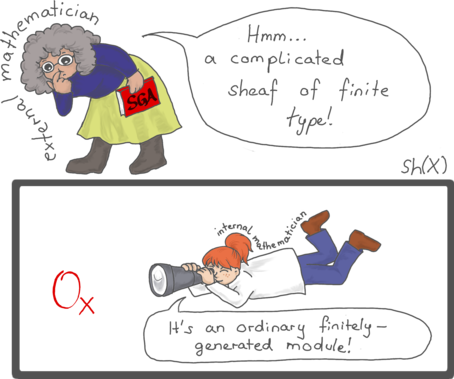
\includegraphics[scale=0.20]{images/external-internal-small}
  \par\medskip\vspace{-0.1em}}
\end{frame}

\backupstart

\begin{frame}
  \slogan{\hil{Understand notions and statements of algebraic geometry
  as notions and statements of algebra internal to appropriate toposes.}}

  {\vspace{-0.1em}\centering
  \rotatebox{90}{\tiny\scalebox{0.5}{Illustration: Carina Willbold}}\hspace{-0.05cm}%
  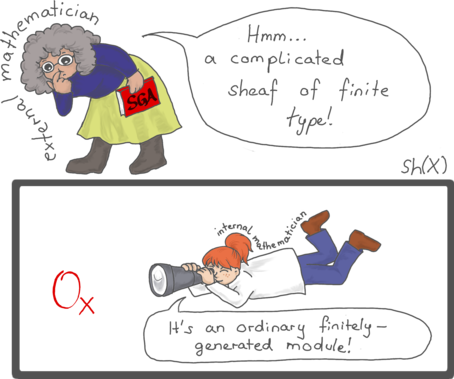
\includegraphics[scale=0.20]{images/external-internal-small}
  \par\medskip\vspace{-0.1em}}

  \begin{itemize}
    \item Simplify proofs and gain conceptual understanding.
    \item Understand relative geometry as absolute geometry.
    \item Develop a synthetic account of scheme theory.
    \item Contribute to constructive algebra.
  \end{itemize}

  \centering
  \hil{\href{http://tiny.cc/topos-notes}{http://tiny.cc/topos-notes}}
  \par
\end{frame}

{\usebackgroundtemplate{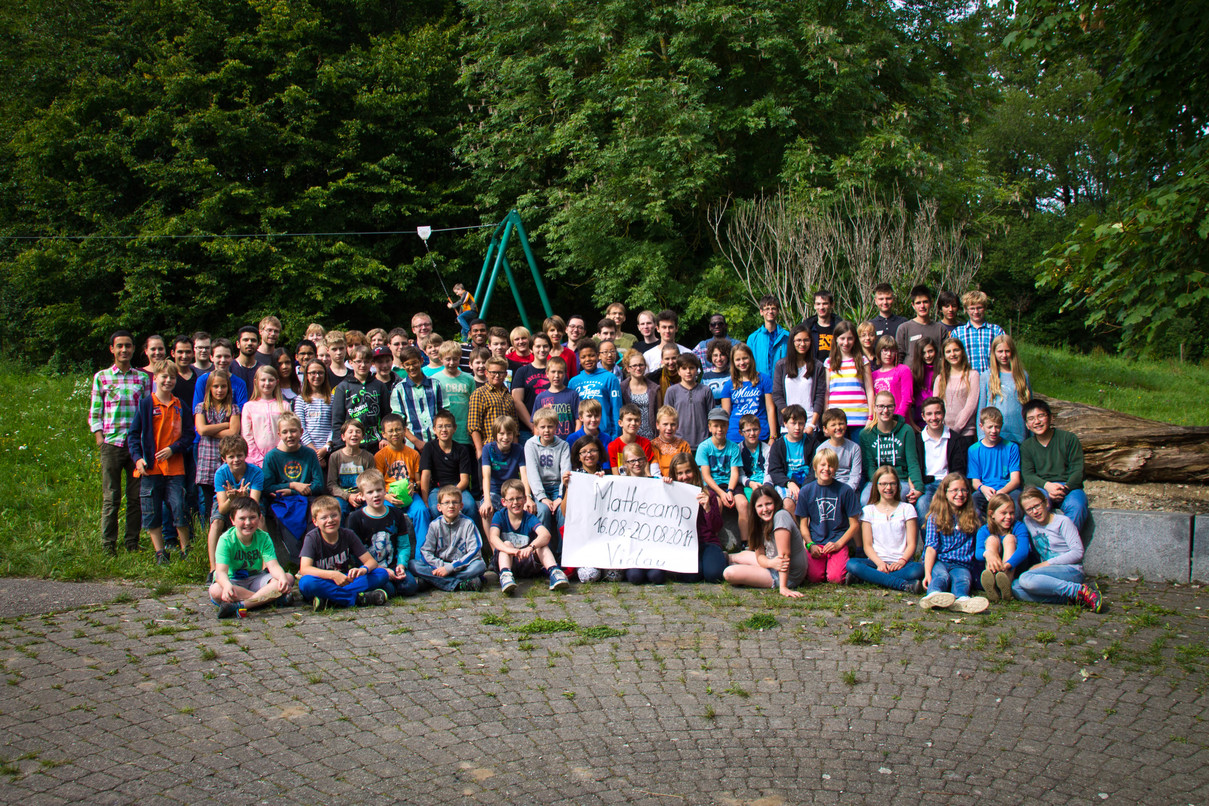
\includegraphics[width=\paperwidth]{images/mathcamp-augsburg}}
\begin{frame}[plain]
  \vspace{\textheight}\vspace{-1em}\centering
  \emph{Participants of Augsburg's maths camp}
  \par
\end{frame}}

{\usebackgroundtemplate{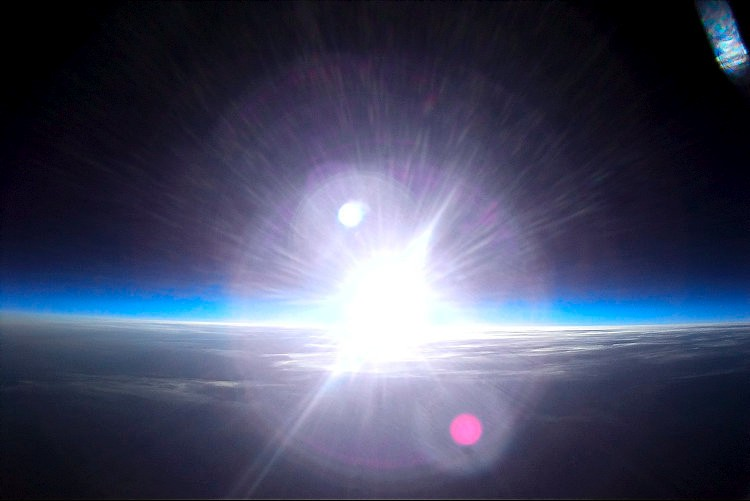
\includegraphics[width=\paperwidth]{images/mathcamp-space}}
\begin{frame}[plain]
  \vspace{\textheight}\vspace{-1em}\centering
  \emph{The sun as seen from our high-altitude balloon}
  \par
\end{frame}}

\appendix

\section{Details on the internal language}

\begin{frame}\frametitle{Translating internal statements I}
  Let~$X$ be a topological space (or locale) and let~$\alpha : \F \to \G$ be a
  morphism of sheaves on~$X$. Then:
  \allowdisplaybreaks
  \begin{align*}
    & \Sh(X) \models \speak{$\alpha$ is surjective} \\[0.5em]
    \Longleftrightarrow\
    & \Sh(X) \models \forall t\?\G\_ \exists s\?\F\_ \alpha(s) = t \\[0.5em]
    \Longleftrightarrow\ &
      \text{for all open~$U \subseteq X$, sections $t \in \G(U)$:} \\
    &\qquad
      \text{there exists an open covering~$U = \textstyle\bigcup_i U_i$ and} \\
    &\qquad
      \text{sections~$s_i \in \F(U_i)$ such that:} \\
    &\qquad\qquad
        \alpha_{U_i}(s_i) = t|_{U_i} \\[0.5em]
    \Longleftrightarrow\ &
      \text{$\alpha$ is an epimorphism of sheaves}
  \end{align*}
\end{frame}

\begin{frame}\frametitle{Translating internal statements II}
  Let~$X$ be a topological space (or locale) and let~$s, t \in \F(X)$ be global
  sections of a sheaf~$\F$ on~$X$. Then:
  \allowdisplaybreaks
  \begin{align*}
    & \Sh(X) \models \neg\neg(s = t) \\[0.5em]
    \Longleftrightarrow\
    & \Sh(X) \models ((s = t) \Rightarrow \bot) \Rightarrow \bot \\[0.5em]
    \Longleftrightarrow\ &
      \text{for all open~$U \subseteq X$ such that} \\
    &\qquad
      \text{for all open~$V \subseteq U$ such that} \\
    &\qquad\qquad
      s|_V = t|_V, \\
    &\qquad
      \text{it holds that~$V = \emptyset$,} \\
    &
      \text{it holds that~$U = \emptyset$} \\[0.5em]
    \Longleftrightarrow\ &
      \text{there exists a dense open set~$W \subseteq X$ such that $s|_W = t|_W$} \\
  \end{align*}
\end{frame}


\section{Spreading from points to neighbourhoods}

\begin{frame}\frametitle{Spreading from points to neighbourhoods}
  All of the following lemmas have a short, sometimes trivial proof.
  Let~$\F$ be a sheaf of finite type on a ringed space~$X$.
  Let~$x \in X$. Let~$A \subseteq X$ be a closed subset. Then:
  \small
  \begin{enumerate}
    \item $\F_x = 0$ iff~$\F|_U = 0$ for some open neighbourhood of~$x$.
    \item $\F|_A = 0$ iff~$\F|_U = 0$ for some open set containing~$A$.
    \item $\F_x$ can be generated by~$n$ elements iff this is true on some open
    neighbourhood of~$x$.
%   \item $\alpha_x$ is surjective iff~$\alpha$ is an epimorphism on some open
%   set containing~$x$, where~$\alpha : \G \to \F$ is any morphism.
    \item $\mathcal{H}\mathrm{om}_{\O_X}(\F,\G)_x \cong
    \Hom_{\O_{X,x}}(\F_x,\G_x)$ if~$\F$ is of finite presentation around~$x$.
    \item $\F$ is torsion iff~$\F_\xi$ vanishes (assume~$X$ integral and~$\F$ quasicoherent).
    \item $\F$ is torsion iff~$\F|_{\mathrm{Ass}(\O_X)}$ vanishes (assume~$X$
    locally Noetherian and~$\F$ quasicoherent).
  \end{enumerate}
\end{frame}

\note{\justifying
  Statements 1 and 2 follow from \emph{one} proof in the internal language,
  applied to two different modal operators.

  Similarly with statements~5 and~6.
  \par
}


\section{The meromorphic functions revisited}

\begin{frame}\frametitle{The smallest dense sublocale}\justifying
  Let~$X$ be a reduced scheme satisfying a technical condition.
  Let~$i : X_{\neg\neg} \to X$ be the inclusion of the smallest dense sublocale
  of~$X$.

  Then~$i_* i^{-1} \O_X \cong \K_X$.

  \begin{itemize}\justifying
    \item This is a highbrow way of saying ``rational functions are regular
    functions which are defined on a dense open subset''.
    \item Another reformulation is that~$\K_X$ is the sheafification of~$\O_X$
    with respect to the~$\neg\neg$-modality.
    \item There is a generalization to nonreduced schemes.
  \end{itemize}
\end{frame}


\subsection{Group schemes}

\begin{frame}\frametitle{Group schemes}
  \hil{Motto:} Internal to~$\Zar(S)$, group schemes look like ordinary groups.
  \bigskip

  \small%
  \begin{tabular}{lll}
    \toprule
    group scheme & internal definition & functor of points: $X \mapsto \ldots$ \\\midrule
    $\GG_\text{a}$ & $\affl$ (as additive group) & $\O_X(X)$ \\[0.5em]
    $\GG_\text{m}$ & $\{ x \? \affl \,|\, \speak{$x$ inv.} \}$ & $\O_X(X)^\times$ \\[0.5em]
    $\mu_n$ & $\{ x \? \affl \,|\, x^n = 1 \}$ & $\{ f \in \O_X(X) \,|\, f^n = 1 \}$ \\[0.5em]
    $\GL_n$ & $\{ M \? \affl^{n \times n} \,|\, \speak{$M$ inv.} \}$ & $\GL_n(\O_X(X))$ \\
    \bottomrule
  \end{tabular}
  \vspace{2em}
\end{frame}


\section{Applications in algebra}

\begin{frame}\frametitle{Applications in algebra}
  Let~$A$ be a commutative ring.
  The internal language of~$\Sh(\Spec A)$ allows you to say ``without loss of
  generality, we may assume that~$A$ is local'', even constructively.

  \begin{center}
    \begin{minipage}{0.75\textwidth}
      \begin{exampleblock}{}
        \justifying
        The kernel of any matrix over a principal ideal domain is finitely
        generated.
      \end{exampleblock}
    \end{minipage}
    \medskip

    \scalebox{3}{$\Downarrow$}

    \begin{minipage}{0.75\textwidth}
      \begin{exampleblock}{}
        \justifying
        The kernel of any matrix over a Prüfer domain is finitely generated.
      \end{exampleblock}
    \end{minipage}
  \end{center}
\end{frame}

\begin{frame}\frametitle{Hilbert's program in algebra}
  \scriptsize\justifying
  There is a way to combine some of the powerful tools of classical ring theory
  with the advantages that constructive reasoning provides, for instance
  exhibiting explicit witnesses. Namely we can devise
  a language in which we can usefully talk about prime ideals, but which
  substitutes non-constructive arguments by constructive arguments ``behind
  the scenes''. The key idea is to substitute the phrase ``for all prime ideals''
  (or equivalently ``for all prime filters'') by ``for the generic prime filter''.

  More specifically, simply interpret a given proof using prime filters
  in~$\Sh(\Spec A)$ and let it refer to~$\F \hookrightarrow \underline{A}$.

  \hspace*{-0.75cm}%
  \begin{tabular}{lll}
    \toprule
    Statement & constructive substitution & meaning \\\midrule
    $x \in \ppp$ for all~$\ppp$. &
    $x \not\in \F$. &
    $x$ is nilpotent. \\
    $x \in \ppp$ for all~$\ppp$ such that~$y \in \ppp$. &
    $x \in \F \Rightarrow y \in \F$. &
    $x \in \sqrt{(y)}$. \\
    $x$ is regular in all stalks~$A_\ppp$. &
    $x$ is regular in~$\ull{A}[\F^{-1}]$. &
    $x$ is regular in~$A$. \\
    The stalks~$A_\ppp$ are reduced. &
    $\ull{A}[\F^{-1}]$ is reduced. &
    $A$ is reduced. \\
    The stalks~$M_\ppp$ vanish. &
    $\ull{M}[\F^{-1}] = 0$. &
    $M = 0$. \\
%   The stalks~$M_\ppp$ are fin.\@ gen.\@ over~$A_\ppp$. &
%   $\ull{M}[\F^{-1}]$ is fin.\@ gen.\@ over
%   $\ull{A}[\F^{-1}]$. &
%   $M$ is fin.\@ gen.\@ over~$A$. \\
    The stalks~$M_\ppp$ are flat over~$A_\ppp$. &
    $\ull{M}[\F^{-1}]$ is flat over~$\ull{A}[\F^{-1}]$. &
    $M$ is flat over~$A$. \\
    The maps~$M_\ppp \to N_\ppp$ are injective. &
    $\ull{M}[\F^{-1}] \to \ull{N}[\F^{-1}]$ is injective. &
    $M \to N$ is injective. \\
    The maps~$M_\ppp \to N_\ppp$ are surjective. &
    $\ull{M}[\F^{-1}] \to \ull{N}[\F^{-1}]$ is surjective. &
    $M \to N$ is surjective. \\
    \bottomrule
  \end{tabular}

  This is related (in a few cases equivalent) to the \emph{dynamical methods in
  algebra} explored by Coquand, Coste, Lombardi, Roy, and others. Their
  approach is more versatile.
  \par
\end{frame}

\backupend

\end{document}
